%%%%%%%%%%%%%%%%%%%%%%%%%%%%%%%%%%%%%%%%%
% Imperial College London Presentation
% LaTeX Template
% Version 1.0 (April 16, 2024)
%
% This template was created by:
% Vel (enquiries@latextypesetting.com)
% LaTeXTypesetting.com
%
%!TEX program = xelatex
% Note: this template must be compiled with XeLaTeX rather than PDFLaTeX
% due to the custom fonts used. The line above should ensure this happens
% automatically, but if it doesn't, your LaTeX editor should have a simple toggle
% to switch to using XeLaTeX.
%
% © Imperial College London, 2024. This template, including logo and fonts, is 
% for use of Imperial staff and students only for university business. All rights 
% reserved to the copyright owners.
%
%%%%%%%%%%%%%%%%%%%%%%%%%%%%%%%%%%%%%%%%%

%----------------------------------------------------------------------------------------
%	CLASS, PACKAGES AND OTHER DOCUMENT CONFIGURATIONS
%----------------------------------------------------------------------------------------

\documentclass[
aspectratio=169, % Uncomment to use an aspect ratio of 16:9 (160 mm by 90 mm)
%aspectratio=43, % Uncomment to use an aspect ratio of 4:3 (128mm by 96mm)
t, % Top align all slide content by default
onlytextwidth, % Typeset content in columns at text width
10pt, % Default font size, use 10pt for the 16:9 aspect ratio and 8pt for the 4:3 aspect ratio
]{beamer}

\usetheme{Imperial} % Use the Imperial theme

%----------------------------------------------------------------------------------------
%	IMPERIAL BEAMER THEME USAGE NOTES
%----------------------------------------------------------------------------------------

% This theme features several predefined Imperial colors which can be used for text and slide backgrounds:
% ICLBlue - Most common slide background color and text color to use (on light backgrounds)
% ICLDarkBlue - Optional darker blue color for slide backgrounds and text
% ICLCream - Accessible background color for use on slide backgrounds
% ICLLightGrey - Accessible background color for use on slide backgrounds

% You can choose to use a 16:9 aspect ratio (default) or a 4:3 aspect ratio by uncommenting the relevant line in the \documentclass specifications above. Note that if you switch between the 2 aspect ratios, you will likely need to adjust how your images are included in the presentation. Usually for a 16:9 aspect ratio, images will be included as width=\paperwidth, but for a 4:3 aspect ratio it's recommended to use height=\paperheight instead.

%----------------------------------------------------------------------------------------
%	PRESENTATION INFORMATION
%----------------------------------------------------------------------------------------

\title{On the subject of lattices} % Presentation title to appear on the title slide and left footers

\subtitle{and why cryptographers love them} % Presentation subtitle to appear on the title slide

\author{Joshua Limbrey} % Author name(s) to appear on the title slide

\date{2024-03-22} % Presentation date to appear on the title slide and right footers


%----------------------------------------------------------------------------------------
%   SET MATHS FONT AND ITALICS
%----------------------------------------------------------------------------------------
\usefonttheme[onlymath]{serif}
\usepackage{newtxtext, newtxmath}
\usepackage{soul} % for strikethrough
\usepackage{multicol}
\usepackage{algorithm}
\usepackage{algpseudocode}
\usepackage{wrapfig}
\usepackage[style=alphabetic,]{biblatex}
\usepackage{amsthm}
\usepackage{tcolorbox}
\usepackage[dvipsnames]{xcolor}

\addbibresource{bib.bib}

%----------------------------------------------------------------------------------------

\begin{document}

%----------------------------------------------------------------------------------------
%	TITLE SLIDES
%----------------------------------------------------------------------------------------

% Select one of the 3 title slide types below and remove or comment out the others

%------------------------------------------------

% Blue background title slide example

\begingroup
\setbeamercolor{background canvas}{bg=ICLBlue} % Slide background color
\setbeamercolor{title page title}{fg=white} % Title text color
\setbeamercolor{title page subtitle}{fg=white} % Subtitle text color
\setbeamercolor{author}{fg=white} % Author(s) text color
\setbeamercolor{date}{fg=white} % Date text color
\setbeamertemplate{title page}[logo]{ICL_Logo_White.pdf} % Imperial logo color, use 'ICL_Logo_White.pdf' for white and 'ICL_Logo_Blue.pdf' for blue
\frame[plain, s]{\titlepage} % Output the title page with no footer ('plain') and vertically distributed text ('s')
\endgroup

%----------------------------------------------------------------------------------------
%	AGENDA SLIDES
%----------------------------------------------------------------------------------------

% White agenda slide

\begingroup
\setbeamercolor{normal text}{fg=ICLBlue}\usebeamercolor[fg]{normal text} % Slide text color

\begin{frame}
    \begin{columns}[T] % [T] ensures correct vertical alignment
        \begin{column}{0.48\linewidth} % Left column
            \HUGE\textbf{Agenda}
        \end{column}
        \begin{column}{0.48\linewidth} % Right column
            \textbf{01}\tabto{0.125\linewidth} What is currently used for cryptography?\\ % Use \tabto{<length>} to add a fixed horizontal whitespace
            \textbf{02}\tabto{0.125\linewidth} What is a lattice?\\
            \textbf{03}\tabto{0.125\linewidth} What are these ``hard lattice problems'?'\\
            \textbf{04}\tabto{0.125\linewidth} What can we do with them?\\
            \textbf{05}\tabto{0.125\linewidth} How we create post quantum schemes?\\
            \textbf{06}\tabto{0.125\linewidth} Some you may have heard of\\
            \textbf{07}\tabto{0.125\linewidth} Where next?\\
            \textbf{08}\tabto{0.125\linewidth} Further reading

        \end{column}
    \end{columns}
\end{frame}
\endgroup

%----------------------------------------------------------------------------------------
%	PRESENTATION BODY SLIDE EXAMPLES
%----------------------------------------------------------------------------------------

\begin{frame}
    \begin{adjustwidth}{0cm}{0.15\textwidth} % The first parameter is the left margin indentation and the second is the right margin indentation
        {\Huge\textcolor{ICLBlue}{{\ImperialSansSemiBold What schemes are currently used for public key cryptography (signatures, key exchanges, etc.) today?}}}
    \end{adjustwidth}
\end{frame}

%------------------------------------------------

\begin{frame}
    \frametitle{What is currently used for cryptography?}

    \begin{columns}[T] % [T] ensures correct vertical alignment
        \begin{column}{0.33\linewidth} % Left column
            \begin{itemize}
                \item Diffie-Hellman
                \item El Gamal
                \item RSA
                \item DSA
                \item ECDSA
                \item ECDH
                \item Ed25519
            \end{itemize}
        \end{column}
        \begin{column}{0.63\linewidth} % Right column
            All public key cryptography relies on what is called a \textbf{trap-door function}.

            Easy to go one way \textit{(encrypt)}, difficult to go the other \textit{(decrypt)} without knowledge of a secret \textit{(private key)}.

            All of the schemes listed to the left are all dependant on the hardness of \textbf{prime factorisation} or the \textbf{discrete logarithm problem}.
        \end{column}
    \end{columns}
\end{frame}

%------------------------------------------------

\begin{frame}
    \frametitle{Why are we bored of these?}
    \begin{columns}[T] % [T] ensures correct vertical alignment
        \begin{column}{0.48\linewidth} % Left column
            These schemes have been around for a while (some nearly 50 years). The security against a standard adversary has been extensively studied, and the hardness of the problems fairly well understood.

            Challenging to construct new and interesting forms of encryption (such as \textit{homomorphic encryption}) due to the properties of the underlying problems.

            Shor's algorithm\footfullcite{shor} means that given an adversary with a sufficiently strong quantum computer, these schemes are no longer secure.
        \end{column}
        \begin{column}{0.48\linewidth} % Right column
            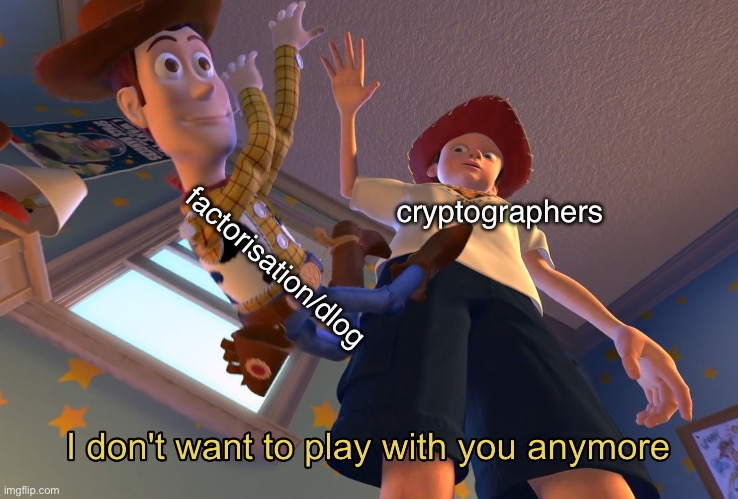
\includegraphics[width=\linewidth]{toy_story.jpeg} % Trimming is used to crop your image and the order of dimensions is: left, bottom, right, top. It's recommended to crop outside of LaTeX though, to ensure the aspect ratio remains the same.
            {\tiny\textcolor{ICLBlue}{(Above) Cryptographers wanting new toys, circa 2000 (colourised)}}
        \end{column}
    \end{columns}
\end{frame}

%------------------------------------------------

\begin{frame}
    \frametitle{What is a lattice?}

    \begin{adjustwidth}{0cm}{0cm} % The first parameter is the left margin indentation and the second is the right margin indentation

        \begin{tcolorbox}[colback=ICLBlue!5!white,colframe=ICLBlue,title=\textbf{Definition:} Lattice]
            The set of all linear integer combinations of basis vectors,
            \[
                \mathcal{L} = \{ \sum_{i = 1}^{d}\mathbf{b}_i\mathbf{x} \ | \ \mathbf{x} \in \mathbb{Z}^d \}
            \]
        \end{tcolorbox}

        \vspace{-0.5em}
        \begin{columns}[T] % [T] ensures correct vertical alignment
            \begin{column}{0.3\linewidth} % Left column
                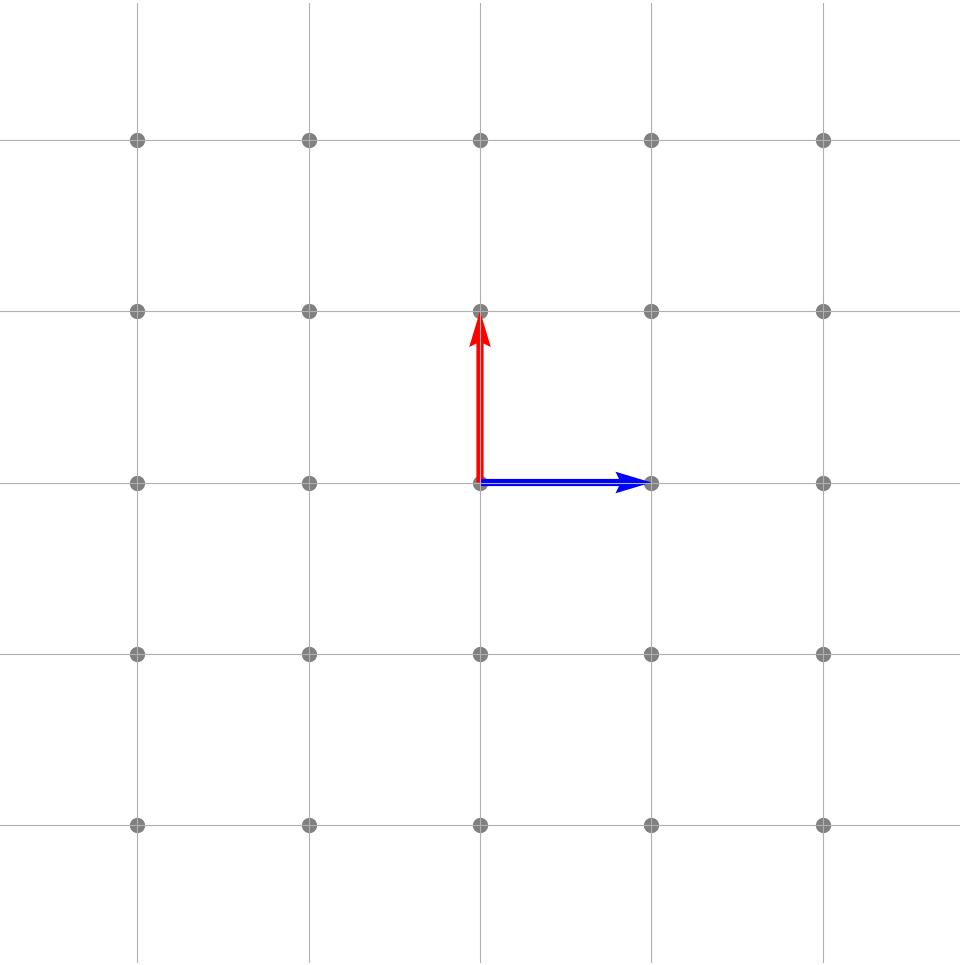
\includegraphics[width=\linewidth]{zn_trivial_basis.jpeg}
            \end{column}
            \begin{column}{0.3\linewidth} % Center column
                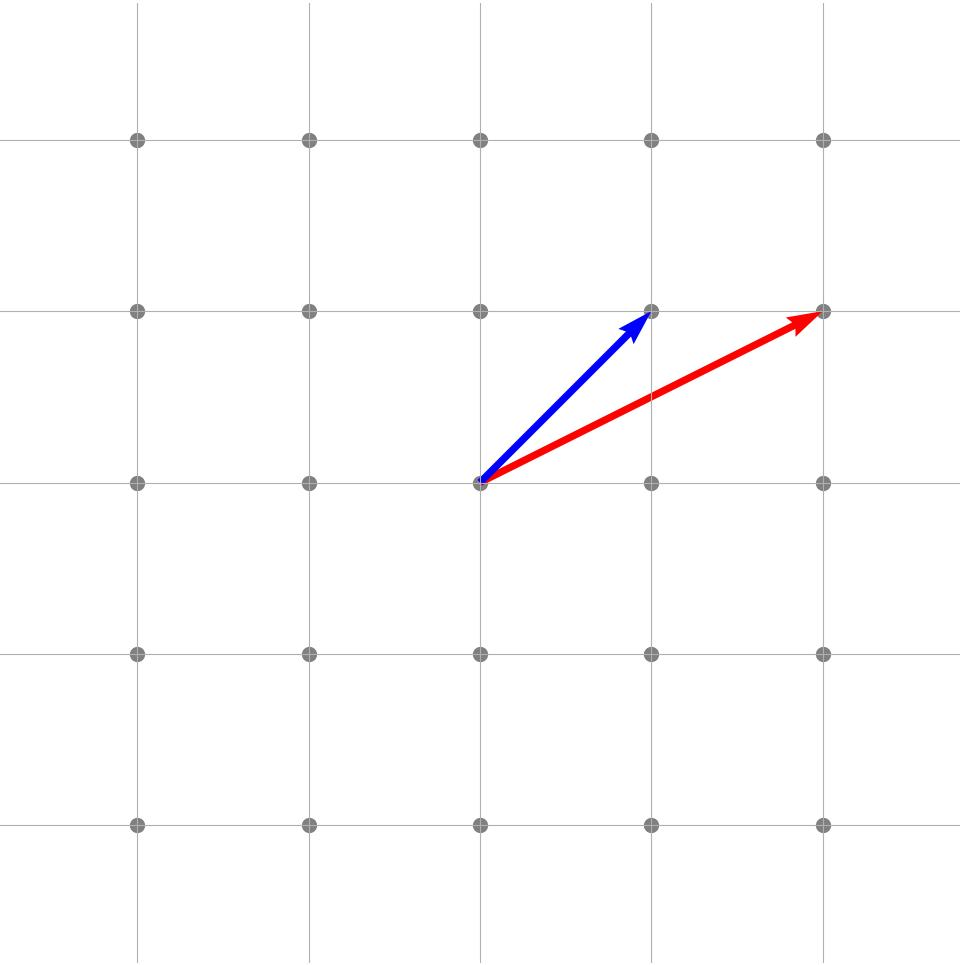
\includegraphics[width=\linewidth]{zn_nontrivial_basis.jpeg}
            \end{column}
            \begin{column}{0.3\linewidth} % Right column
                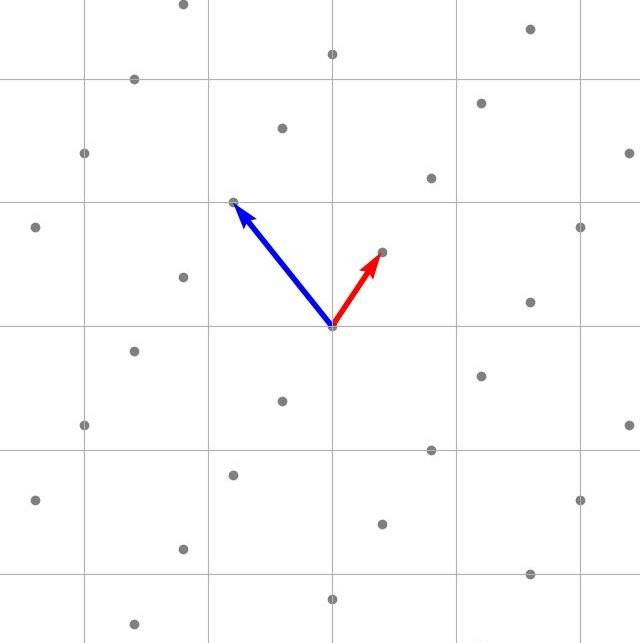
\includegraphics[width=\linewidth]{Figure_1.jpeg}
            \end{column}
        \end{columns}
    \end{adjustwidth}
\end{frame}

%------------------------------------------------

\begin{frame}
    \frametitle{What are hard lattice problems?}

    \begin{adjustwidth}{0cm}{0cm} % The first parameter is the left margin indentation and the second is the right margin indentation

        \begin{tcolorbox}[colback=ICLBlue!5!white,colframe=ICLBlue,title=\textbf{Definition:} Shortest Vector Problem (SVP)]
            Given a lattice, find the shortest \textit{non-zero} lattice point.
        \end{tcolorbox}

        \begin{tcolorbox}[colback=ICLBlue!5!white,colframe=ICLBlue,title=\textbf{Definition:} Learning With Errors Problem (LWE)]
            Let, $\color{ForestGreen} \begin{bmatrix} \\ \mathbf{b} \\ \\ \end{bmatrix} \color{black} = \color{ForestGreen} \begin{bmatrix} & & \\ & \mathbf{A} & \\ & & \end{bmatrix} \color{black} \begin{bmatrix} \\ \mathbf{s} \\ \\ \end{bmatrix} + \begin{bmatrix} \\ \mathbf{e} \\ \\ \end{bmatrix}$.
            Knowing \textit{only} the values in \color{ForestGreen} green\color{black}, find $\begin{bmatrix} \\ \mathbf{s} \\ \\ \end{bmatrix}$.
        \end{tcolorbox}
        \begin{tcolorbox}[colback=ICLBlue!5!white,colframe=ICLBlue,title=\textbf{Definition:} Lattice Isomorphism Problem (LIP)]
            Given two lattices, $\mathcal{L}_1$ and $\mathcal{L}_2$, find the scaling factor and rotation to send one to the other (if it exists).
        \end{tcolorbox}

        But we also have the Short Integer Solutions problem (SIS), the NTRU problem, the Closest Vector Problem (CVP), and all the many variants of anything mentioned here!

    \end{adjustwidth}
\end{frame}

%------------------------------------------------

\begin{frame}
    \frametitle{Shortest/Closest Vector Problem}
    \begin{columns}[T] % [T] ensures correct vertical alignment
        \begin{column}{0.48\linewidth} % Left column
            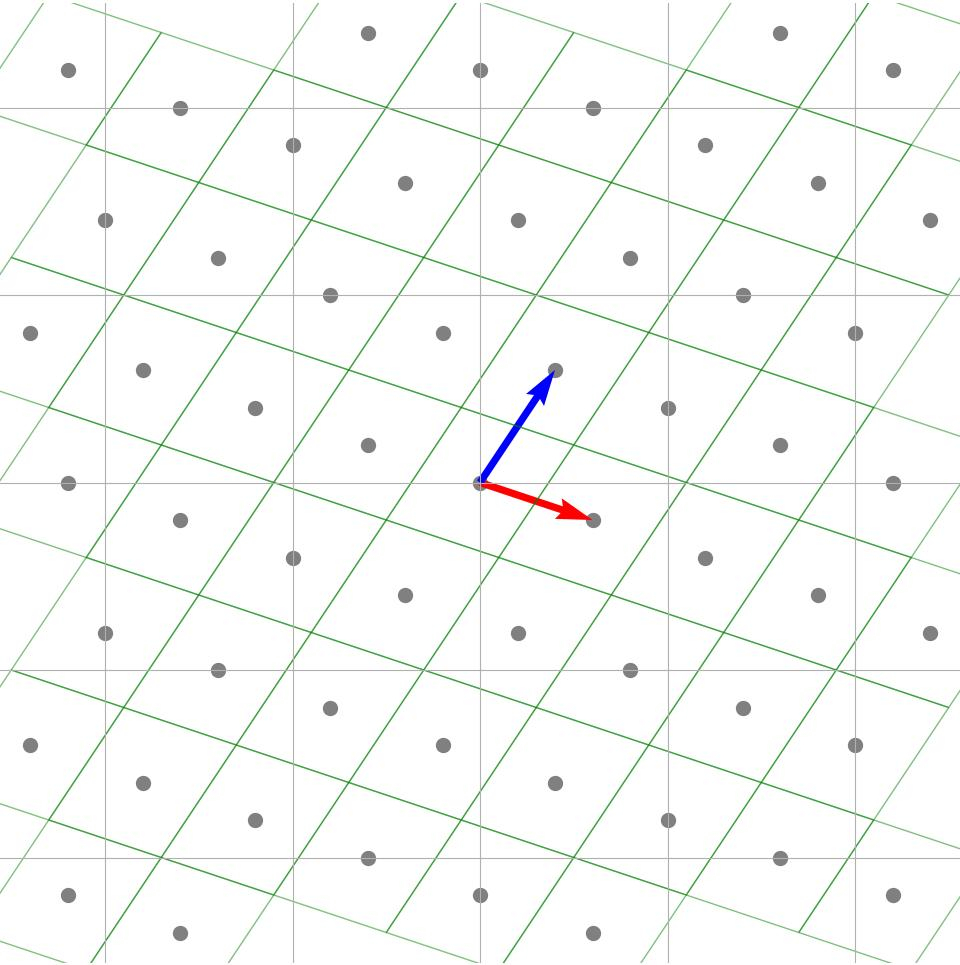
\includegraphics[width=\linewidth]{good_basis_svp.jpeg} % Trimming is used to crop your image and the order of dimensions is: left, bottom, right, top. It's recommended to crop outside of LaTeX though, to ensure the aspect ratio remains the same.
        \end{column}
        \begin{column}{0.48\linewidth} % Right column
            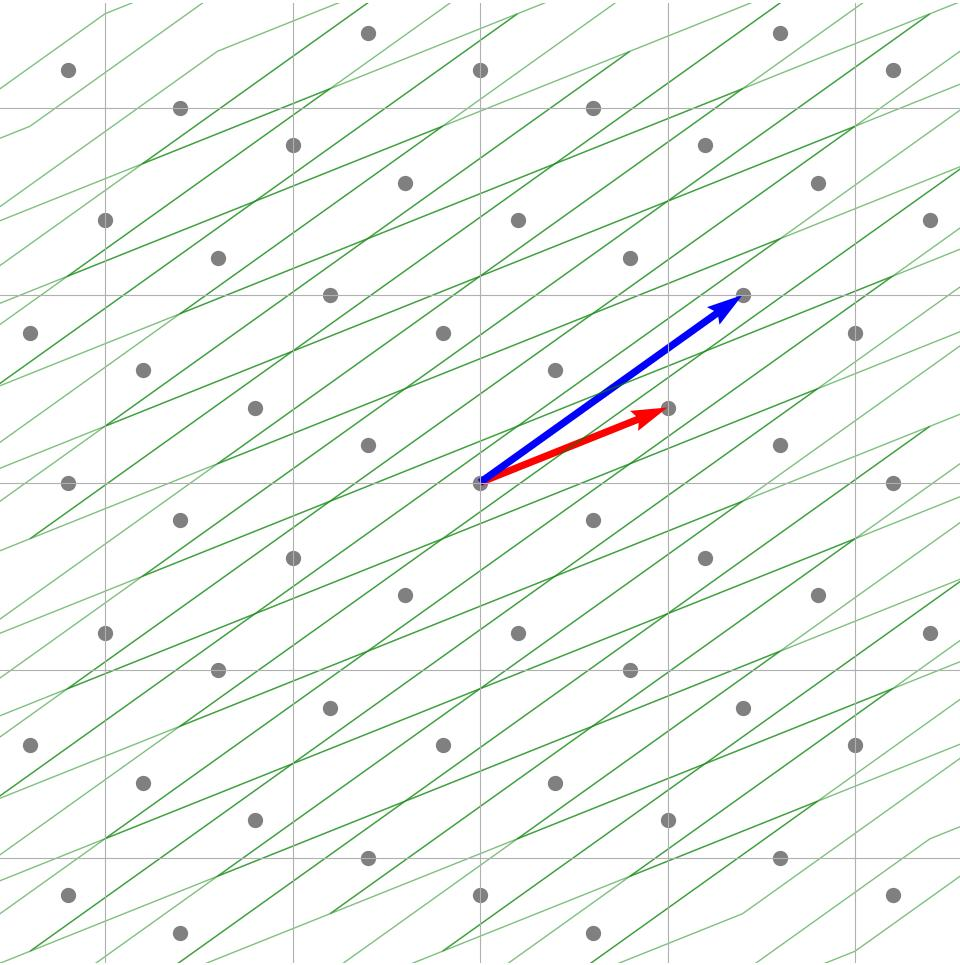
\includegraphics[width=\linewidth]{bad_basis_svp.jpeg} % Trimming is used to crop your image and the order of dimensions is: left, bottom, right, top. It's recommended to crop outside of LaTeX though, to ensure the aspect ratio remains the same.
        \end{column}
    \end{columns}
\end{frame}

%------------------------------------------------

\begin{frame}
    \frametitle{Learning With Errors}
    \begin{columns}[T] % [T] ensures correct vertical alignment
        \begin{column}{0.48\linewidth} % Left column
            \begin{tcolorbox}[colback=ICLBlue!5!white,colframe=ICLBlue,title=Learning With Errors Problem (LWE)]
                \[
                    \color{ForestGreen} \begin{bmatrix} \\ \mathbf{b} \\ \\ \end{bmatrix} \color{black} = \color{ForestGreen} \begin{bmatrix} & & \\ & \mathbf{A} & \\ & & \end{bmatrix} \color{red} \begin{bmatrix} \\  \mathbf{s} \\ \\ \end{bmatrix} \color{black} + \begin{bmatrix} \\ \mathbf{e} \\ \\ \end{bmatrix}
                \]
            \end{tcolorbox}

            We can construct what is called a $q$-ary lattice using $\mathbf{A}$.

            Then, taking the target vector $\mathbf{b}$, solving a CVP instance \textit{should} give us $\mathbf{As}$, and therefore $\mathbf{s}$.

            Unfortunately, if the LWE parameters are chosen well, we do not get a good basis for our new lattice, and so solving CVP is hard.
        \end{column}
        \begin{column}{0.48\linewidth} % Right column
            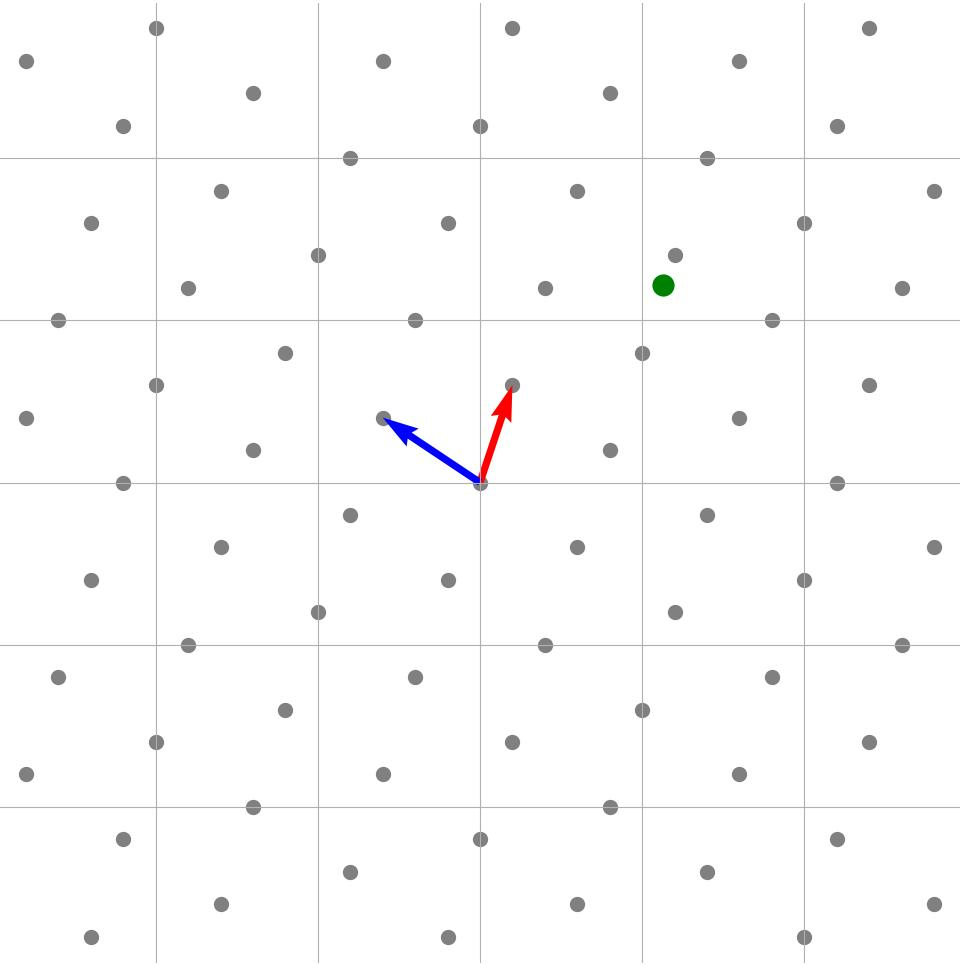
\includegraphics[width=\linewidth]{lwe_lattice.jpeg} % Trimming is used to crop your image and the order of dimensions is: left, bottom, right, top. It's recommended to crop outside of LaTeX though, to ensure the aspect ratio remains the same.
        \end{column}
    \end{columns}
\end{frame}

%------------------------------------------------

\begin{frame}
    \frametitle{Learning With Errors}
    \begin{columns}[T] % [T] ensures correct vertical alignment
        \begin{column}{0.48\linewidth} % Left column
            \begin{tcolorbox}[colback=ICLBlue!5!white,colframe=ICLBlue,title=Learning With Errors Problem (LWE)]
                \[
                    \color{ForestGreen} \begin{bmatrix} \\ \mathbf{b} \\ \\ \end{bmatrix} \color{black} = \color{ForestGreen} \begin{bmatrix} & & \\ & \mathbf{A} & \\ & & \end{bmatrix} \color{red} \begin{bmatrix} \\  \mathbf{s} \\ \\ \end{bmatrix} \color{black} + \begin{bmatrix} \\ \mathbf{e} \\ \\ \end{bmatrix}
                \]
            \end{tcolorbox}

            With a good basis for our lattice, something that can be kept secret, solving CVP and recovering the secret is easy, however.

            In practice, we have methods of turning a bad basis into a good basis (\textit{lattice reduction}), but these algorithms do not scale well for high dimension lattices.
        \end{column}
        \begin{column}{0.48\linewidth} % Right column
            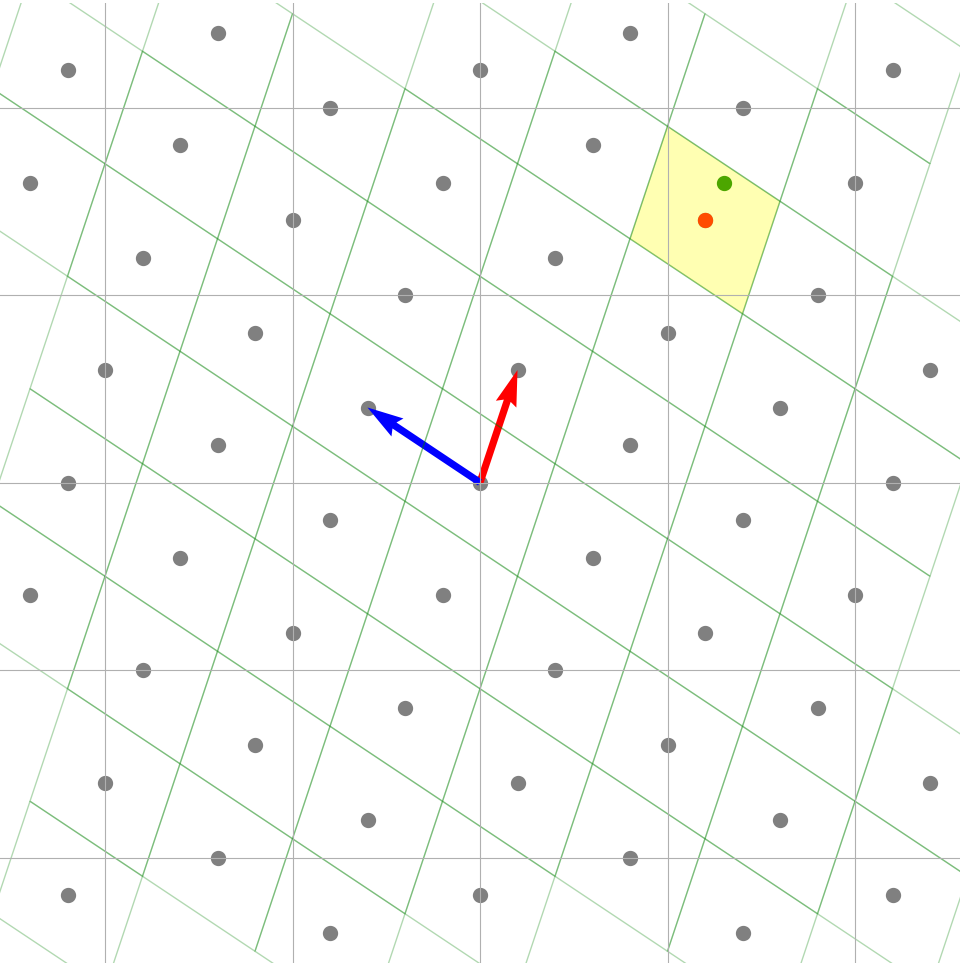
\includegraphics[width=\linewidth]{lwe_lattice_solved.png} % Trimming is used to crop your image and the order of dimensions is: left, bottom, right, top. It's recommended to crop outside of LaTeX though, to ensure the aspect ratio remains the same.
        \end{column}
    \end{columns}
\end{frame}

%------------------------------------------------

\begin{frame}
    \frametitle{Lattice Isomorphism Problem}
    \begin{columns}[T] % [T] ensures correct vertical alignment
        \begin{column}{0.48\linewidth} % Left column
            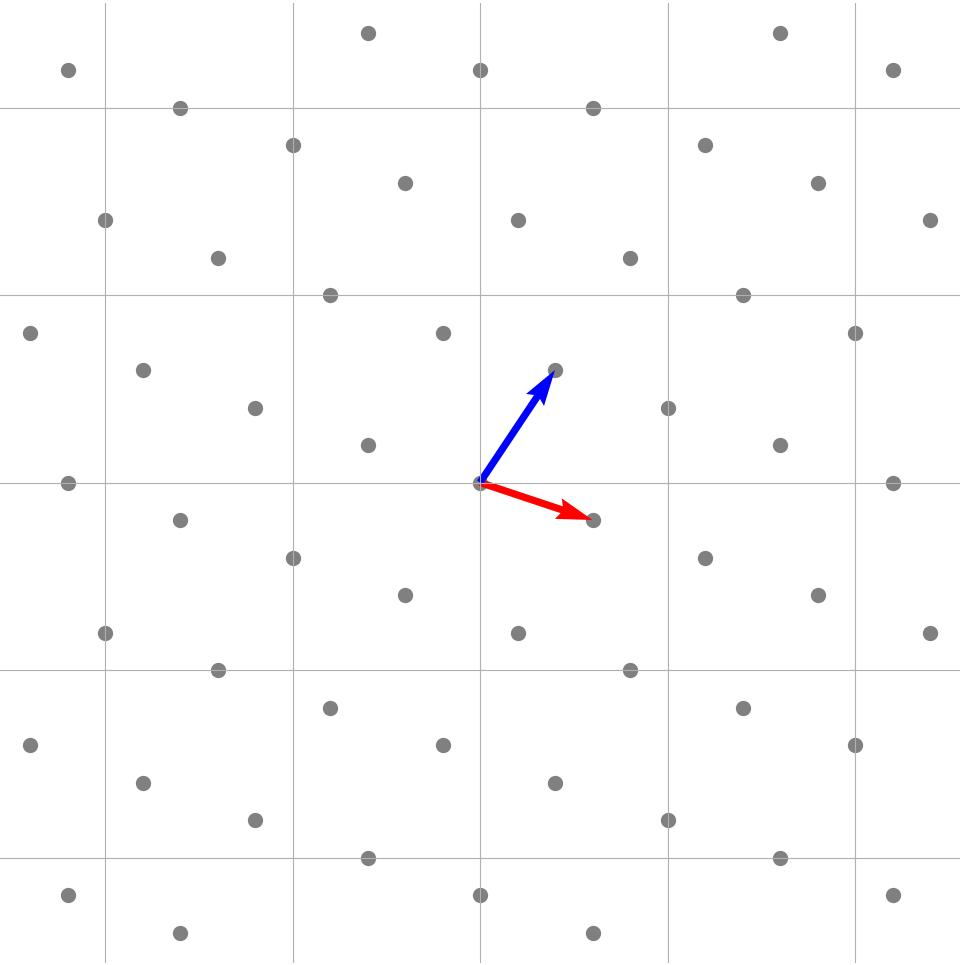
\includegraphics[width=\linewidth]{lip_instance.jpeg} % Trimming is used to crop your image and the order of dimensions is: left, bottom, right, top. It's recommended to crop outside of LaTeX though, to ensure the aspect ratio remains the same.
        \end{column}
        \begin{column}{0.48\linewidth} % Right column
            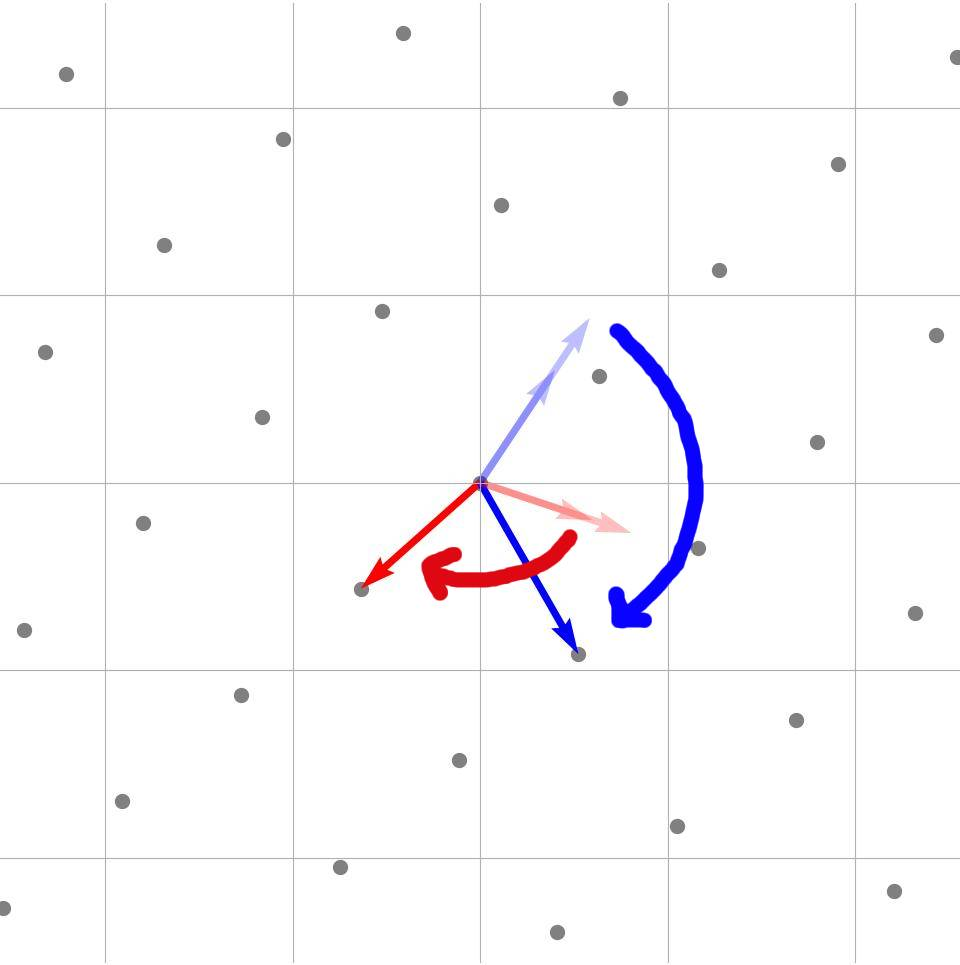
\includegraphics[width=\linewidth]{lip_instance_alt.jpeg} % Trimming is used to crop your image and the order of dimensions is: left, bottom, right, top. It's recommended to crop outside of LaTeX though, to ensure the aspect ratio remains the same.
        \end{column}
    \end{columns}
\end{frame}


%------------------------------------------------

\begin{frame}
    \frametitle{It's all SVP?}

    \begin{columns}[T] % [T] ensures correct vertical alignment
        \begin{column}{0.58\linewidth} % Left column
            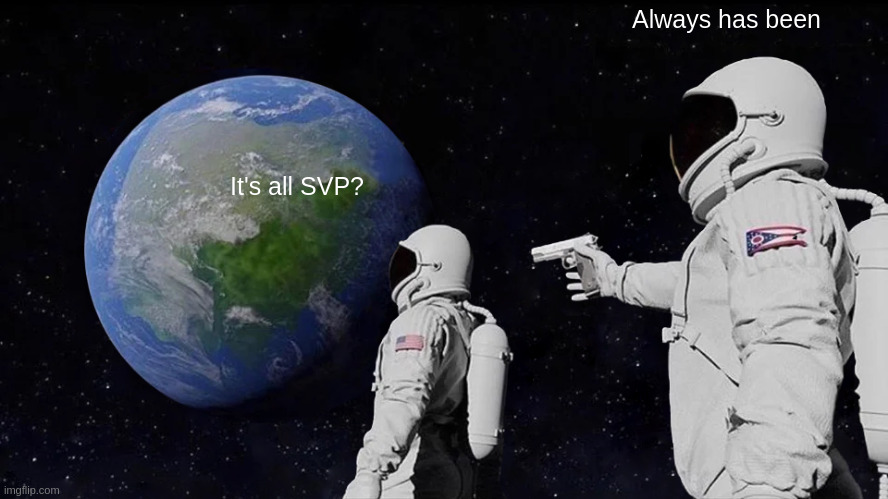
\includegraphics[width=0.9\linewidth]{always_has_been.jpg} % Trimming is used to crop your image and the order of dimensions is: left, bottom, right, top. It's recommended to crop outside of LaTeX though, to ensure the aspect ratio remains the same.

            \vspace{-1.5em}{\tiny\textcolor{ICLBlue}{(Above) Regev discovering the the LWE to $\gamma$-SVP reduction, 2005}}\newline

            \vspace{-2em}But don't worry, even though all of these problems are reducible to SVP, they all work in slightly different ways, giving the schemes we build from them different properties (speed, key size, etc.).
        \end{column}
        \begin{column}{0.38\linewidth} % Right column
            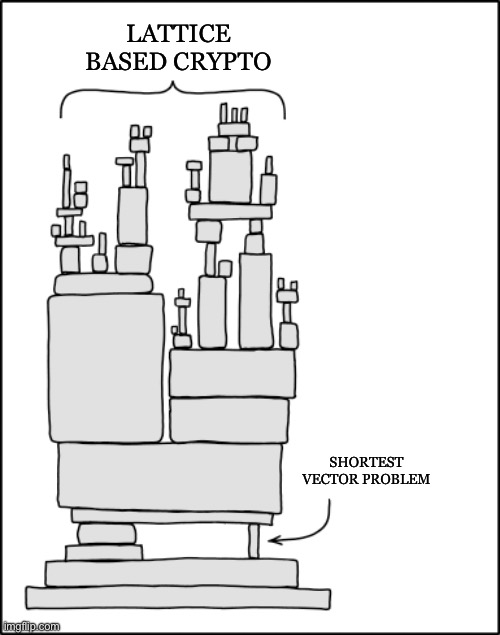
\includegraphics[width=0.85\linewidth]{svp_crutch.jpeg} % Trimming is used to crop your image and the order of dimensions is: left, bottom, right, top. It's recommended to crop outside of LaTeX though, to ensure the aspect ratio remains the same.

            \vspace{-1.5em}{\tiny\textcolor{ICLBlue}{(Above) xkcd Dependency, lattice based cryptography special edition}}
        \end{column}
    \end{columns}
\end{frame}

%------------------------------------------------

\begin{frame}
    \frametitle{What can we do with lattices?}

    % Top-left quarter
    \begin{minipage}[t][0.45\textheight][t]{0.48\linewidth}
        \textbf{Fully Homomorphic Encryption}\\
        FHE allows computations to be applied on encrypted data without needing to be decrypted first. This allows a user to allow a semi-trusted third party to operate on their data, without being able to access it, in such a way that when the user decrypts their data the same operations have been applied to the plaintext.
    \end{minipage}%
    \hfill
    % Top-right quarter
    \begin{minipage}[t][0.45\textheight][t]{0.48\linewidth}
        \textbf{Cryptanalysis of Classical Schemes}\\
        Lattices are also used by cryptographers when attacking classical schemes such as RSA and ECC. They typically exploit weaknesses in parameter generation and utilise the collection of many signed messages by a single key\footfullcite{classical}.
    \end{minipage}
    

    \vspace{-1.5em}
    % Bottom-left quarter
    \begin{minipage}[t][0.45\textheight][t]{0.48\linewidth}
        \textbf{Secure Multiparty Computation}\\
        Similar to FHE, MPC is a privacy preserving construct in which a number of participants all want to compute a value as a public function of each of their private data. MPC allows them to do so whilst maintaining the secrecy of their inputs.
    \end{minipage}
    \hfill
    % Bottom-right quarter
    \begin{minipage}[t][0.2\textheight][t]{0.48\linewidth}
        \vspace{3.5em}
        \textbf{Post-Quantum Cryptography}\\
        It is believed that these lattice problems are hard to solve even on quantum computers.
    \end{minipage}
\end{frame}

%------------------------------------------------

\begin{frame}
    \frametitle{Some schemes you may have heard of}
    \framesubtitle{LWE Based}

    \begin{columns}[T] % [T] ensures correct vertical alignment
        \begin{column}{0.42\linewidth} % Left column
            \textbf{ML-KEM/Kyber and ML-DSA/Dilithium}\\
            
            ML-KEM\footfullcite{mlkem}/DSA\footfullcite{mldsa} were both elected by NIST as schemes for standardisation, with the standards published August 2024. These are both front runners due to their speed, however their drawback is a fairly large key size. LWE is a well studied assumption, with strong worst and average case analysis.
        \end{column}
        \begin{column}{0.55\linewidth} % Right column
            \textbf{Where Can I Find This?}\\
            \begin{itemize}
                \item Cloudflare now support x25519xML-KEM in CIRCL\footnote{https://blog.cloudflare.com/post-quantum-to-origins/}
            \item Chrome supports x25519xML-KEM as default for TLS\footnote{https://blog.chromium.org/2023/08/protecting-chrome-traffic-with-hybrid.html}
                \item liboqs, the open-quantum-safe x Microsoft fork of openTLS supports ML-KEM and ML-DSA\footnote{https://github.com/open-quantum-safe/liboqs}
                \item As of release 9.9, OpenSSH supports mlkem768x25519-sha256 by default\footnote{https://www.openssh.com/releasenotes.html}
                \item Amazon supports ML-KEM in hybrid in AWS Key Management Service\footnote{https://aws.amazon.com/kms/}
            \end{itemize}
        \end{column}
    \end{columns}
\end{frame}

%------------------------------------------------

\begin{frame}
    \frametitle{Some schemes you may have heard of}
    \framesubtitle{NTRU Based}

    \begin{columns}[T] % [T] ensures correct vertical alignment
        \begin{column}{0.42\linewidth} % Left column
            \textbf{Falcon and NTRUPrime}\\
            
            Falcon\footfullcite{falcon} was selected as a digital signature scheme by NIST, however is yet to be standardised. NTRUPrime\footfullcite{ntruprime} was not selected for standarisation by NIST, but is another popular key encapsulation scheme.
        \end{column}
        \begin{column}{0.55\linewidth} % Right column
            \textbf{Where Can I Find This?}\\
            \begin{itemize}
                \item liboqs, the open-quantum-safe x Microsoft fork of openTLS supports Falcon and NTRUPrime\footnote{https://github.com/open-quantum-safe/liboqs}
                \item As of release 9.9, OpenSSH supports sntrup761x25519-sha512 by default\footnote{https://www.openssh.com/releasenotes.html}
            \end{itemize}
        \end{column}
    \end{columns}
\end{frame}

%------------------------------------------------

\begin{frame}
    \frametitle{Some schemes you may have heard of}
    \framesubtitle{LIP Based}

    \begin{columns}[T] % [T] ensures correct vertical alignment
        \begin{column}{0.58\linewidth} % Left column
            \textbf{HAWK}\\
            
            Hawk\footfullcite{hawk} is the youngest of all schemes listed, and is currently the only lattice based scheme left in NISTs call for additional signature schemes\footfullcite{nistsig}. HAWKs biggest selling points are smaller keys and signatures compared to other (LWE) signature schemes whilst maintaining the speed of lattices.
        \end{column}
        \begin{column}{0.4\linewidth} % Right column
            \textbf{Where Can I Find This?}\\
            \begin{itemize}
                \item No where I could find yet...
            \end{itemize}
        \end{column}
    \end{columns}
\end{frame}


%------------------------------------------------

\begin{frame}
    \frametitle{What if I don't want to use lattices?}

    \begin{adjustwidth}{0cm}{0cm} % The first parameter is the left margin indentation and the second is the right margin indentation
        There are plenty of other foundations for PQC such as isogenies, cubic forms, and codes. In some cases, these might solve some issues we have with lattices \textit{(key and signature size)}, but often with the trade-off of lattice benefits \textit{(speed)}.

        They can also let us create cool new applications, in the same way that lattices allow us to create fully homomorphic encryption, such as non-interactive key exchanges and verifiable delay functions.

        Their biggest selling point is that they're based on different hard problems - if SVP is broken in the same way that factoring was, we have something else to fall back on.
    \end{adjustwidth}
\end{frame}

%----------------------------------------------------------------------------------------
%	CLOSING SLIDES
%----------------------------------------------------------------------------------------

% Blue closing slide

\begingroup
	\setbeamercolor{background canvas}{bg=ICLBlue} % Slide background color
	\setbeamercolor{normal text}{fg=white}\usebeamercolor[fg]{normal text} % Slide text color
	\setbeamertemplate{closing slide logo}[logo]{ICL_Logo_White.pdf} % Imperial logo color, use 'ICL_Logo_White.pdf' for white and 'ICL_Logo_Blue.pdf' for blue
	\setbeamertemplate{closing slide text}[text]{Thank you} % Slide text
	
	\usebeamertemplate{closing slide} % Output the closing slide
\endgroup

%----------------------------------------------------------------------------------------

\end{document}
